\documentclass[10pt]{article}

% -------------------------
% PAQUETES
% -------------------------
\usepackage[spanish]{babel}
\usepackage[utf8]{inputenc}
\usepackage[T1]{fontenc}
\usepackage{geometry}
\usepackage{setspace}
\usepackage{graphicx}
\usepackage{amsmath}
\usepackage{booktabs}
\usepackage{caption}
\usepackage{hyperref}
\usepackage{apacite}
\usepackage{microtype}

% -------------------------
% CONFIGURACION DE PAGINA
% -------------------------
\geometry{
 top=1.5cm,
 left=1.5cm,
 right=1.5cm,
 bottom=2cm
}
\setstretch{1.0}
\setlength{\parindent}{0pt}
\setlength{\parskip}{0.5em}

% -------------------------
% FIGURAS / TABLAS
% -------------------------
\captionsetup{font=small, labelfont=bf}
\renewcommand{\figurename}{Fig.}
\renewcommand{\tablename}{Tabla}

% El proyecto mantiene las secciones y la bibliografía dentro de `informe/`.
% Las figuras quedan en `resultados/` porque ese directorio sí está en la raíz.
\graphicspath{{resultados/}}

% -------------------------
% IDENTIFICACION DE GRUPO
% -------------------------
\title{\textbf{Analisis PCA del Boston Housing}}

\author{
Natalay Huaiquinao, Carlos Ulloa\\
\texttt{nhuaiquinao2021@alu.uct.cl, carlos.ulloa2020@alu.uct.cl}
}

\date{\vspace{-0.6em}Tarea 4, INFO1184, Semestre I-2026}

% -------------------------
\begin{document}

\maketitle
\vspace{-1.0cm}

\begin{abstract}
Este trabajo analiza el conjunto de datos Boston del paquete MASS siguiendo las fases 1 a 5 de CRISP-DM y usando An\'alisis de Componentes Principales como t\'ecnica central. Primero se describen las variables, se verifican valores faltantes y se detectan valores at\'ipicos en varias columnas, con presencia clara en 
\textit{black}, 
\textit{zn}, 
\textit{crim}, 
\textit{medv}, 
\textit{chas}, 
\textit{rm}, 
\textit{ptratio}, 
\textit{lstat} y 
\textit{dis}. Luego se estandarizan las variables explicativas y se ajusta un PCA, donde el primer componente explica 51.06\% de la varianza y cinco componentes alcanzan 80\% acumulado. En la fase de evaluaci\'on se responde que el tama\~no de la vivienda influye positivamente en el precio, que la cercan\'ia al r\'io Charles tambi\'en se asocia con valores mayores, que el estatus socioecon\'omico tiene efecto negativo marcado y que la criminalidad puede modelarse con variables socioecon\'omicas y espaciales. El informe integra evidencia gr\'afica y num\'erica para sustentar cada conclusi\'on.
\end{abstract}

\section{Introduccion}
El problema se centra en el an\'alisis del conjunto de datos Boston, disponible en \texttt{MASS}, con el objetivo de describir su estructura, identificar patrones relevantes y responder las preguntas de investigaci\'on formuladas en la tarea. La metodolog\'ia se organiza seg\'un CRISP-DM en las fases de comprensi\'on del negocio, comprensi\'on de los datos, preparaci\'on, modelado y evaluaci\'on, dejando la implementaci\'on computacional como soporte reproducible del estudio.

El objetivo general es caracterizar los factores asociados al valor mediano de las viviendas y explorar si el PCA ayuda a sintetizar la informaci\'on multivariada. Como objetivos espec\'ificos se busca detectar at\'ipicos, identificar los suburbios con menor valor de vivienda, cuantificar la relaci\'on entre el n\'umero de habitaciones y el precio, evaluar el efecto de \textit{chas} y \textit{lstat}, y revisar si la tasa de criminalidad puede explicarse a partir de otras variables. El documento se organiza en fundamentos te\'oricos, desarrollo metodol\'ogico, discusi\'on, conclusiones y anexo.

\section{Fundamentos de teoria}
CRISP-DM propone una secuencia pr\'actica para proyectos de miner\'ia de datos: comprender el negocio, comprender los datos, prepararlos, modelar y evaluar los resultados antes de comunicar conclusiones \citeA{crispdm2000}. En este caso, la fase de negocio se traduce en preguntas sobre precios de vivienda, criminalidad y condiciones socioecon\'omicas.

El An\'alisis de Componentes Principales (PCA) es una t\'ecnica de reducci\'on de dimensionalidad que transforma un conjunto de variables correlacionadas en nuevas variables ortogonales llamadas componentes principales \citeA{jolliffe2016}. Su utilidad radica en condensar informaci\'on sin perder excesiva varianza y en revelar estructuras latentes entre variables. Dado que las variables del Boston Housing tienen escalas distintas, la estandarizaci\'on es obligatoria antes de aplicar PCA. Las cargas de cada componente permiten interpretar qu\'e variables dominan la estructura del fen\'omeno, mientras que los scores resumen la posici\'on de cada observaci\'on en el espacio reducido.

El paquete \texttt{MASS} provee el conjunto de datos y forma parte de la tradici\'on estad\'istica aplicada en R \citeA{masspackage,venables2002}. En consecuencia, el an\'alisis combina estad\'istica descriptiva, visualizaci\'on y modelamiento lineal para justificar cada respuesta.

\section{Desarrollo del trabajo}
\subsection{Fase 1: comprensi\'on del negocio}
La tarea busca explicar el comportamiento del precio de vivienda \textit{medv} y su relaci\'on con variables estructurales, ambientales y socioecon\'omicas. El enfoque se limita a las fases 1 a 5 de CRISP-DM porque el producto esperado es un informe anal\'itico y no un sistema en producci\'on.

\subsection{Fase 2: comprensi\'on de los datos}
El conjunto Boston contiene 506 observaciones y 14 variables. No se detectaron valores faltantes, pero s\'i outliers en varias columnas, lo que confirma distribuciones asim\'etricas y colas largas. La Fig.~\ref{fig:outliers} resume este comportamiento.

\begin{figure}[htbp]
    \centering
    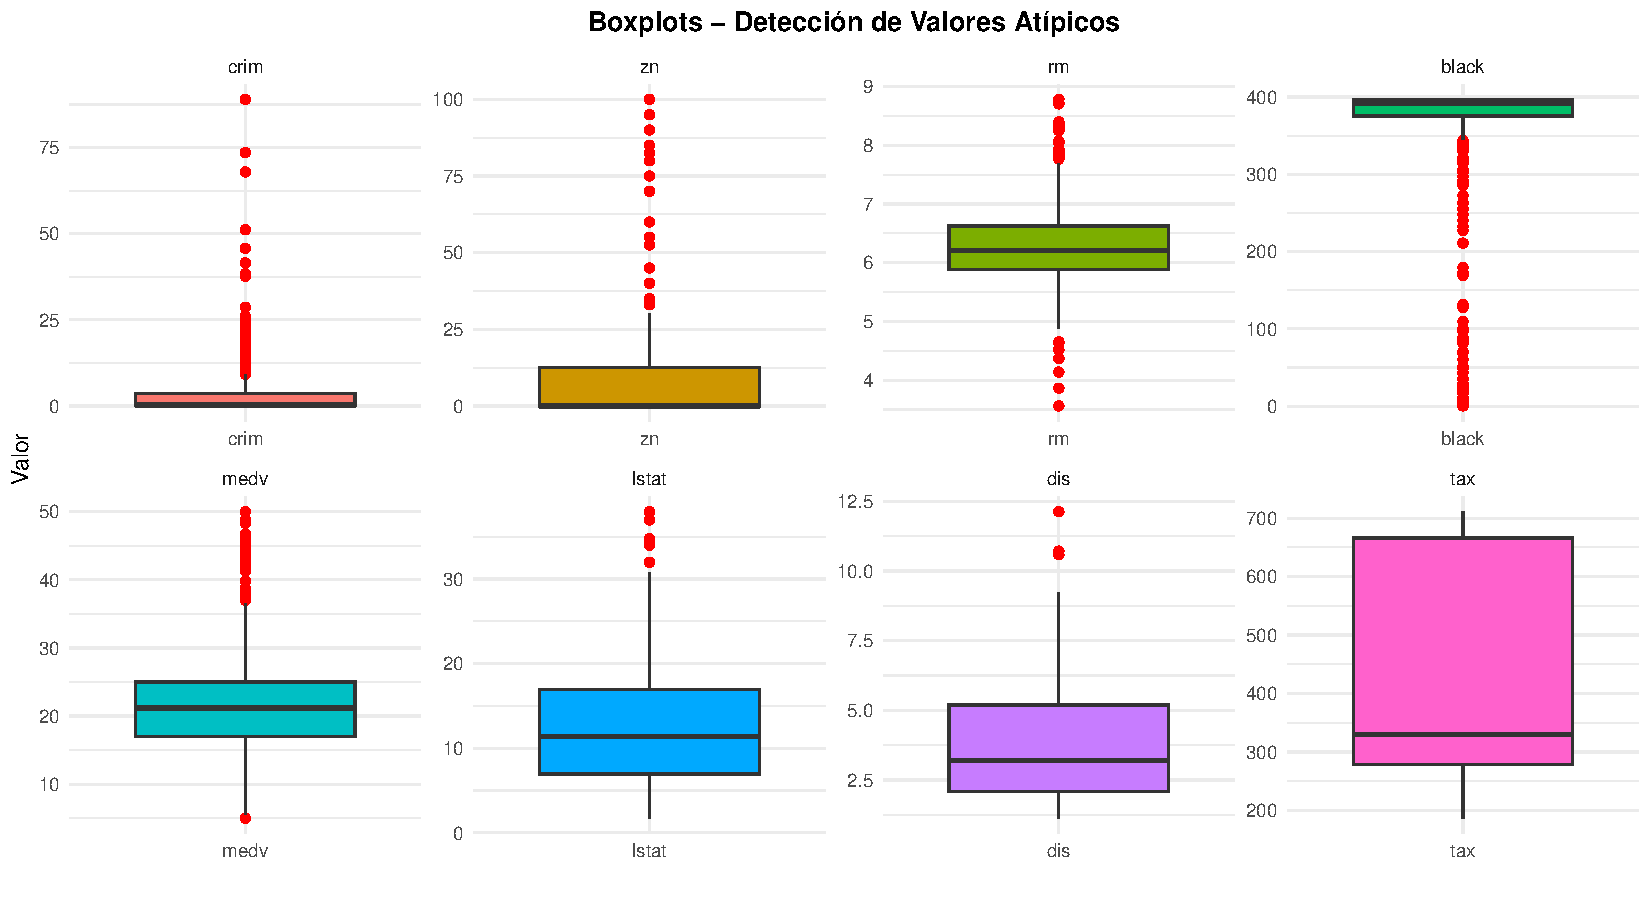
\includegraphics[width=0.9\textwidth]{boxplots_outliers.pdf}
    \caption{Detecci\'on visual de valores at\'ipicos en variables seleccionadas.}
    \label{fig:outliers}
\end{figure}

La matriz de correlaci\'on muestra relaciones fuertes entre variables urbanas y socioecon\'omicas, especialmente entre \textit{rad} y \textit{tax}, y una asociaci\'on negativa marcada entre \textit{lstat} y \textit{medv}. Esto sugiere que el valor de la vivienda est\'a vinculado a la condici\'on social del entorno.

\subsection{Fase 3: preparaci\'on de los datos}
Para el PCA se excluyeron \textit{chas} y \textit{medv} del bloque explicativo, porque la primera es una variable binaria contextual y la segunda es la variable de inter\'es principal. Luego se estandarizaron las 12 variables restantes para evitar que la escala dominara la soluci\'on.

\subsection{Fase 4: modelado PCA}
El scree plot confirma que el primer componente explica 51.06\% de la varianza y que cinco componentes acumulan 80\%. Esto permite reducir la dimensionalidad sin perder informaci\'on esencial.

La estructura de cargas indica que PC1 concentra principalmente variables asociadas a urbanizaci\'on y presi\'on urbana, como \textit{indus}, \textit{nox}, \textit{rad}, \textit{tax}, \textit{age} y \textit{lstat}, mientras que \textit{rm} y \textit{dis} se mueven en sentido contrario. En t\'erminos interpretativos, PC1 puede leerse como un gradiente de deterioro/urbanizaci\'on versus calidad residencial. Este resultado es consistente con la varianza explicada: PC1 aporta 51.06\% y cinco componentes concentran m\'as de 80\%.

\subsection{Fase 5: evaluaci\'on de las preguntas}
La pregunta sobre suburbios m\'as baratos se responde con el ranking de \textit{medv}: las observaciones 399, 406, 401, 400 y 415 est\'an entre las de menor valor, con precios entre 5.0 y 7.0. La Tabla~\ref{tab:respuestas} sintetiza las evidencias principales para cada pregunta.

\begin{table}[htbp]
\centering
\small
\begin{tabular}{p{2.0cm}p{4.9cm}p{5.0cm}}
\toprule
Pregunta & Evidencia principal & Conclusi\'on \\
\midrule
P1 & Outliers en al menos ocho variables, con mayor presencia en \textit{black}, \textit{zn} y \textit{crim}. & S\'i existen valores at\'ipicos. \\
P2 & Menores valores de \textit{medv} en las observaciones 399, 406, 401, 400 y 415. & Hay suburbios claramente m\'as baratos. \\
P3 & Correlaci\'on \textit{rm-medv} = 0.6954 y pendiente positiva significativa. & M\'as habitaciones implica mayor precio. \\
P4 & Media de \textit{medv}: 22.09 si \textit{chas}=0 y 28.44 si \textit{chas}=1; $p=0.003567$. & La cercan\'ia al r\'io eleva el valor. \\
P5 & Correlaci\'on \textit{lstat-medv} = -0.7377 y R$^2$ = 0.5441. & El estatus socioecon\'omico bajo reduce el valor. \\
P6 & Modelo con \textit{rad, tax, lstat, dis, medv, indus, nox} logra R$^2$ = 0.4337; con scores PCA y \textit{PC1--PC4}, R$^2$ = 0.6126. & La criminalidad es explicable en parte y el PCA ayuda a resumirla. \\
\bottomrule
\end{tabular}
\caption{S\'intesis de resultados para las preguntas de investigaci\'on.}
\label{tab:respuestas}
\end{table}

La relaci\'on entre tama\~no de la vivienda y precio es fuerte y positiva, como muestra la Fig.~\ref{fig:rmmedv}. Del mismo modo, la comparaci\'on por \textit{chas} evidencia diferencias estad\'isticamente significativas en \textit{medv}, por lo que la cercan\'ia al r\'io Charles no parece ser neutral para el mercado inmobiliario.

\begin{figure}[htbp]
    \centering
    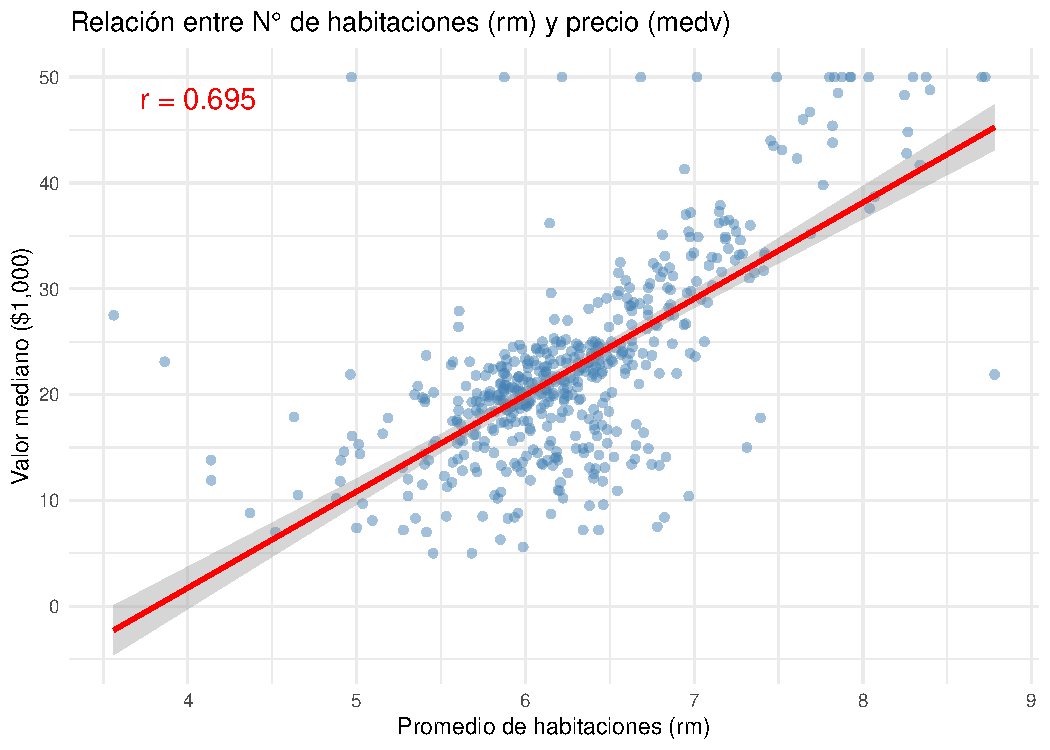
\includegraphics[width=0.84\textwidth]{relacion_rm_medv.pdf}
    \caption{Relaci\'on entre el n\'umero medio de habitaciones y el valor de la vivienda.}
    \label{fig:rmmedv}
\end{figure}

\begin{figure}[htbp]
    \centering
    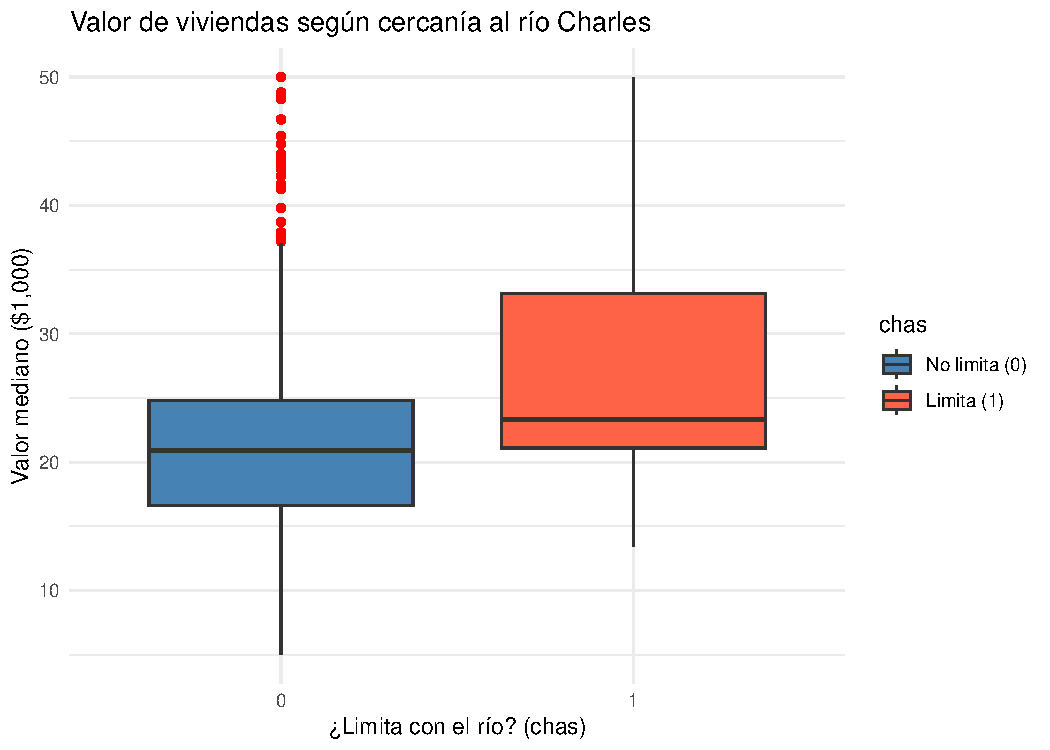
\includegraphics[width=0.82\textwidth]{boxplot_medv_chas.pdf}
    \caption{Valor de viviendas seg\'un cercan\'ia al r\'io Charles.}
    \label{fig:chas}
\end{figure}

En cuanto a \textit{lstat}, la relaci\'on negativa es una de las m\'as fuertes del conjunto y confirma que el nivel socioecon\'omico del entorno es un predictor relevante del precio. Finalmente, para \textit{crim} se observa que variables como \textit{rad}, \textit{dis}, \textit{lstat} y \textit{medv} aportan informaci\'on estad\'isticamente significativa, mientras que el modelo basado en componentes principales mejora la capacidad explicativa global.

\section{Discusion y reflexion}
Los resultados son coherentes con la l\'ogica econ\'omica del problema: viviendas con m\'as habitaciones tienden a costar m\'as, mientras que zonas con mayor proporci\'on de poblaci\'on de bajo estatus socioecon\'omico presentan menores valores de mercado. La variable \textit{chas} muestra un efecto positivo, pero con una muestra muy desbalanceada entre los casos 0 y 1, por lo que conviene interpretar la diferencia con cautela.

El PCA result\'o \textit{útil} para reducir dimensionalidad y resumir la estructura del conjunto, aunque no reemplaza el an\'alisis inferencial de variables puntuales. Su fortaleza aqu\'i es exploratoria: permite visualizar agrupamientos y detectar qu\'e variables dominan el comportamiento conjunto. Como limitaci\'on, el modelo lineal para \textit{crim} puede verse afectado por colinealidad entre predictores, por lo que una extensi\'on natural ser\'ia validar el ajuste con subconjuntos de entrenamiento/prueba o con regularizaci\'on.

Otra limitaci\'on importante es que en la pregunta de suburbios m\'as baratos no se dispone de nombres geogr\'aficos, sino de identificadores de observaci\'on; por eso el informe debe hablar de observaciones o suburbios indexados, no de barrios con nombre propio. Aun as\'i, el an\'alisis permite responder las preguntas con evidencia suficiente y reproducible.

\section{Conclusiones}
\subsection*{Conclusi\'on de Natalay Huaiquinao}
Se logr\'o aplicar CRISP-DM sobre el conjunto Boston, identificar outliers, preparar los datos, ejecutar PCA y responder las preguntas de investigaci\'on con evidencia cuantitativa. El aprendizaje principal fue distinguir entre una reducci\'on de dimensionalidad para exploraci\'on y un modelo predictivo para explicar variables objetivo.

\subsection*{Conclusi\'on de Carlos Ulloa}
El an\'alisis confirma que el precio de vivienda est\'a muy relacionado con el n\'umero de habitaciones, el estatus socioecon\'omico y la cercan\'ia al r\'io Charles, mientras que la criminalidad se puede aproximar con variables urbanas y socioecon\'omicas. Como mejora futura, conviene complementar el estudio con validaci\'on predictiva y un tratamiento m\'as formal de at\'ipicos.

\section{Referencias}
\bibliographystyle{apacite}
\bibliography{informe/referencias}

\appendix
\section{Anexo}
En el anexo se recomienda dejar la evidencia completa del desarrollo computacional, sin saturar el cuerpo principal del informe. Los archivos generados por el script que respaldan el an\'alisis son, entre otros, \texttt{boxplots	extunderscore outliers.pdf}, \texttt{scree	extunderscore plot.pdf}, \texttt{relacion	extunderscore rm	extunderscore medv.pdf}, \texttt{boxplot	extunderscore medv	extunderscore chas.pdf}, \texttt{relacion	extunderscore lstat	extunderscore medv.pdf}, \texttt{regresion	extunderscore medv	extunderscore rm.txt}, \texttt{regresion	extunderscore medv	extunderscore lstat.txt}, \texttt{regresion	extunderscore multiple	extunderscore crim.txt} y \texttt{respuestas	extunderscore preguntas.txt}.

\subsection{Bit\'acora de trabajo}
\begin{itemize}
    \item D\'ia 1: revisi\'on del enunciado, carga del dataset Boston y exploraci\'on inicial.
    \item D\'ia 2: limpieza, estandarizaci\'on, PCA y generaci\'on de figuras/tablas.
    \item D\'ia 3: interpretaci\'on de resultados, redacci\'on del informe y validaci\'on final.
\end{itemize}

\end{document}